\documentclass{../../myassignment}

\courselabel{MAT110}
\exercisesheet{Assignment 2}{}

\usepackage{amssymb}
\usepackage{amsmath}
%\usepackage{bm}
\usepackage{mathtools}
\usepackage{xfrac}
\newcommand{\uvec}[1]{\boldsymbol{\hat{\textbf{#1}}}}
\allowdisplaybreaks
\renewcommand*{\arraystretch}{1.5}

\begin{document}
	\begin{problem}
		Regn ut flateintegralet $$\iint_T x dS$$ der $T$ er delen av sfæren $x^2+y^2+z^2=a^2$ som ligger i første oktant $x\geq0, y\geq0, z\geq0$.
	\end{problem}

	\begin{answer}
		\begin{align*}
			&\iint_T f dS = \iint_A f(\vec{r}(\theta,\varphi))\vert(\frac{\partial\vec{r}}{\partial \theta}\times{\frac{\partial \vec{r}}{\partial \varphi}})(\theta, \varphi)\vert  d \theta d \varphi \\[1cm]
			%
			&\vec{r}(u,v) = a \cdot \sin(\varphi)\cos(\theta) \uvec{\i} + a \cdot \sin(\varphi)\sin(\theta) \uvec{\j} + a \cdot \cos(\varphi)\uvec{k}\\[1cm]
			%
			&\therefore \iint_T x dS = \iint_A (a \cdot \sin(\varphi)\cos(\theta))\vert(\frac{\partial\vec{r}(\theta, \varphi)}{\partial \theta}\times{\frac{\partial \vec{r}(\theta, \varphi)}{\partial \varphi}})\vert  d \theta d \varphi \\[1cm]
			%
			&= \iint_A (a \cdot \sin(\varphi)\cos(\theta)) \vert
				\begin{pmatrix}
					-a\sin(\varphi)\sin(\theta) \\
					a\sin(\varphi)\cos(\theta) \\
					0
				\end{pmatrix} \times 
				\begin{pmatrix}
					a\cos(\varphi)\cos(\theta) \\
					a\cos(\varphi)\sin(\theta) \\
					-a\sin(\varphi)
				\end{pmatrix}
					\vert  d \theta d \varphi \\[1cm]
				%
				&= \iint_A (a \cdot \sin(\varphi)\cos(\theta)) \vert
				\begin{vmatrix}
					\uvec{\i} & \uvec{\j} & \uvec{k}\\
					-a\sin(\varphi)\sin(\theta) &
						a\sin(\varphi)\cos(\theta) &
						0 \\
					a\cos(\varphi)\cos(\theta) &
						a\cos(\varphi)\sin(\theta) &
						-a\sin(\varphi)
				\end{vmatrix}
					\vert  d \theta d \varphi \\[1cm]
				%
				&= \iint_A (a \cdot \sin(\varphi)\cos(\theta)) \vert
				\uvec{k}
				\begin{vsmallmatrix}
					-a\sin(\varphi)\sin(\theta) &
						a\sin(\varphi)\cos(\theta) \\
					a\cos(\varphi)\cos(\theta) &
						a\cos(\varphi)\sin(\theta) &
				\end{vsmallmatrix}
				-a\sin(\varphi)
				\begin{vsmallmatrix}
					\uvec{\i} & \uvec{\j}\\
					-a\sin(\varphi)\sin(\theta) &
						a\sin(\varphi)\cos(\theta) &
				\end{vsmallmatrix}
				\vert  d \theta d \varphi \\[1cm]
				%
				&= \iint_A (a \cdot \sin(\varphi)\cos(\theta)) \vert
				\uvec{k} (
					-a^2\sin\varphi\cos\varphi\sin^2\theta - 
					a^2\sin\varphi\cos^2\theta\cos\varphi
				) \\* &\hspace{3cm}
				-a\sin\varphi (
					\uvec{\i} a\sin\varphi\cos\theta + \uvec{\j}a\sin\varphi\sin\theta
				)
				\vert  d \theta d \varphi \\[1cm]
				%
				&= \iint_A (a \cdot \sin(\varphi)\cos(\theta)) \vert
				\begin{pmatrix}
					-a^2\sin^2\varphi\cos\theta  \\
					-a^2\sin^2\varphi\sin\theta \\
					-a^2\sin\varphi\cos\varphi
				\end{pmatrix}
				\vert  d \theta d \varphi\\[1cm]
				%
				&= \iint_A (a \cdot \sin(\varphi)\cos(\theta)) \sqrt{
					(-a^2\sin^2\varphi\cos\theta)^2 +
					(-a^2\sin^2\varphi\sin\theta)^2 +
					(-a^2\sin\varphi\cos\varphi)^2}
				 d \theta d \varphi\\[1cm]
				%
				&= \iint_A (a \cdot \sin(\varphi)\cos(\theta)) \sqrt{
					a^4\sin^4\varphi\cos^2\theta +
					a^4\sin^4\varphi\sin^2\theta +
					a^4\sin^2\varphi\cos^2\varphi}
				 d \theta d \varphi\\[1cm]
				%
				&= \iint_A (a \cdot \sin(\varphi)\cos(\theta)) \sqrt{a^4\sin^2\varphi (\sin^2\varphi + \cos^2\varphi)}\\
				&= \iint_A (a \cdot \sin(\varphi)\cos(\theta)) \sqrt{a^4\sin^2(\varphi)}  d\theta d\varphi \\
				&= \iint_A a^3 \cdot \sin^2(\varphi)\cos(\theta) d\theta d\varphi \\
				&= \int_0^{\sfrac{\tau}{4}} \left[\int_0^{\sfrac{\tau}{4}} a^3 \cdot \sin^2(\varphi)\cos(\theta)  d\varphi\right]  d\theta \\
				&= a^3 \int_0^{\sfrac{\tau}{4}} \cos(\theta) \left[\int_0^{\sfrac{\tau}{4}} \sin^2(\varphi)  d\varphi\right]  d\theta \\
				&= a^3 \int_0^{\sfrac{\tau}{4}} \cos(\theta) \left[ \frac{\varphi-\sin(\varphi)\cos(\varphi)}{2} \right]_0^{\sfrac{\tau}{4}}  d\theta \\
				&= a^3 \int_0^{\sfrac{\tau}{4}} \cos(\theta) \frac{{\sfrac{\tau}{4}}-\sin({\sfrac{\tau}{4}})\cos({\sfrac{\tau}{4}})}{2}  d\theta \\
				&= a^3 \int_0^{\sfrac{\tau}{4}} \cos(\theta) \frac{\tau}{8}  d\theta =
				 \frac{\tau a^3}{8}  \left[ \sin(\theta) \right]_0^{\sfrac{\tau}{4}} \\[1cm]
				&= \frac{\tau a^3}{8}
		\end{align*}
		Overflatearealet til planet i kule-domenet er altså $\sfrac{a^3\tau}{8}$, der $a$ er radiusen til kula vår.

	\end{answer}

	\pagebreak
	\begin{problem}
		En dobbelt deriverbar funksjon $f:\mathbb{R}^2\to\mathbb{R}$ kalles harmonisk dersom den tilfredstiller Laplace-likningen $$\frac{\partial^2f}{\partial x^2}+\frac{\partial^2f}{\partial y^2}=0$$.
			\begin{itemize}
				\item Vis at funskjonene $x^4-6x^2y^2+y^4$ og $e^xsin(y)$ er harmoniske.
				\item Vis at dersom $f$ er harmonisk, så er $$\int_C (\frac{\partial f}{\partial y}dx - \frac{\partial f}{\partial x}dy) = 0$$ for alle enkle, lukkede, glatte kurver $C$ i planet.
			\end{itemize}
	\end{problem}
	\begin{answer}
		\begin{eqnarray*}
			\frac{\partial^2f}{\partial x^2}+\frac{\partial^2f}{\partial y^2} &=& 0 \\
			\frac{\partial^2 (x^4-6x^2y^2+y^4)}{\partial x^2}+\frac{\partial^2 (x^4-6x^2y^2+y^4)}{\partial y^2} &=& 0 \\
			\frac{\partial (4x^3-12xy^2)}{\partial x}+\frac{\partial (-12x^2y+4y^3)}{\partial y} &=& 0 \\
			(12x^2-12y^2) + (-12x^2+12y^2) &=& 0 \\
			(x^2-y^2) + (-x^2+y^2) &=& 0 \\
			0 &=& 0
		\end{eqnarray*}

	\end{answer}
	\begin{answer}
		\begin{eqnarray*}
			\frac{\partial^2f}{\partial x^2}+\frac{\partial^2f}{\partial y^2} &=& 0 \\
			\frac{\partial^2 (e^x sin(y))}{\partial x^2}+\frac{\partial^2 (e^x sin(y))}{\partial y^2} &=& 0 \\
			\frac{\partial (e^x sin(y))}{\partial x}+\frac{\partial (e^x cos(y))}{\partial y} &=& 0 \\
			(e^x sin(y)) + (-e^x sin(y)) &=& 0 \\
			0 &=& 0 \\
		\end{eqnarray*}
		Begge funskjonene er dermed harmoniske.

	\end{answer}

	\pagebreak
	\begin{answer}
		Green's teorem sier at $\int_C P dx + Q dy = \iint_R (\frac{\partial Q}{\partial x} - \frac{\partial P}{\partial y}) dxdy$ er gyldig for alle enkle, lukkede og glatte kurver C. 

		Ved å erstatte $P=\frac{\partial f}{\partial y}$ og $Q=\frac{\partial f}{\partial x}$, og ved å bruke definisjonen til harmonisk funskjon har vi:
		\begin{align*}
			\int_C P dx + Q dy &= \iint_R (\frac{\partial Q}{\partial x} - \frac{\partial P}{\partial y}) dxdy \\[1cm]
			\int_C \frac{\partial f}{\partial y} dx + \frac{\partial f}{\partial x} dy &= \iint_R (\frac{\partial Q}{\partial x} - \frac{\partial P}{\partial y}) dxdy \\[1cm]
			\int_C \frac{\partial f}{\partial y} dx + \frac{\partial f}{\partial x} dy &= \iint_R (\frac{\partial \frac{\partial f}{\partial x}}{\partial x} - \frac{\partial \frac{\partial f}{\partial y}}{\partial y}) dxdy \\[1cm]
			\int_C \frac{\partial f}{\partial y} dx + \frac{\partial f}{\partial x} dy &= \iint_R (\frac{\partial^2 f}{\partial x^2} - \frac{\partial^2 f}{\partial y^2}) dxdy \\[1cm]
			%	\text{Siden vi vet at $(\frac{\partial^2 f}{\partial x^2} - \frac{\partial^2 f}{\partial y^2})$ er like null følger:}\\
			\int_C \frac{\partial f}{\partial y} dx + \frac{\partial f}{\partial x} dy &= \iint_R 0 dxdy \\
			\int_C \frac{\partial f}{\partial y} dx + \frac{\partial f}{\partial x} dy &= 0 \\
		\end{align*}

		Siden vi integrerer på et domene vet vi at svarer blir null uten noen konstanter, og har dermed bevist hypotesen.

	\end{answer}

	\pagebreak
	\begin{problem}
		La $A = [-1,1]\times[-1,1]$ og la $\vec{F} : A \to \mathbb{R}^2$ være gitt ved $$\vec{F}(x,y)=\frac{1}{5}(xy+y^2-1, \,x^3-y^2+3).$$

		\begin{itemize}
			\item Vis at $\vec{F}$ definerer en funskjon $\vec{F} : A \to A$ (altså at verdiene til $\vec{F}$ ligger i $A$).
			\item Vis at $\vec{F} : A \to A$ definerer en kontraksjon. (Hint: Setning 5.5.8 i boka (gjengitt nedenfor) kan bli nyttig her).
			\item Vis at følgenende likningsystem har en unik løsning for $-1 \leq x,y \leq 1$: 
				\begin{eqnarray*}
					5x &=& xy + y^2 - 1 \\
					5y &=& x^3 - y^2 + 3.
				\end{eqnarray*}
			\item Lag et MATLAB/Python script som regner ut en approksimasjon til løsningen i c) ved hjelp av en iterasjon $x_{n+1} = \vec{F}(x_n)$. Programmet skal ta startpunkt $x_0$ og antall iterasjoner som input. Legg ved et plott av følgende du får med startpunkt i $(0,0)$ og $(-1,1)$.
		\end{itemize}

	\end{problem}

	\begin{answer}
		For at $\vec{F} : A \to A$ skal være sant må $f_x(x,y) = \frac{1}{5}(xy+y^2), \{x \in [-1, 1] \land y \in [-1,1]\}$ gi et tall mellom $-1$ og $1$. Det samme gjelder for $f_y(x,y) = \frac{1}{5}(x^3 - y^2 + 3)$. 

		Det er trivielt at de høyeste verdiene av $|F_x|$ må være en del av $x,y$-parene $(1,-1), (1,1), (-1,-1), (-1,1)$, som gir $F_x = \frac{1}{5}\{-1, 1, 1, -1\}$. Disse verdiene ligger under domenet $A_x$. Vi har dermed bevist at $F_x : A_x \to A_x$. 

		På samme måte ser vi at $|F_y|$ har samme patent. Med samme verdiene får vi $F_y = \frac{1}{5}\{3, 3, 1, 1\}$. Siden vi nå vet at både $F_x$ og $F_y$ er en del av A, vet vi at $F : A \to A$ er gyldig for alle verdiene i $F$.

	\end{answer}

	\pagebreak
	\begin{answer}
		\begin{align}
			\vec{F}(x,y) = \frac{1}{5}\begin{pmatrix}
				xy+y^2-1 \\ 
				x^3-y^2+3
			\end{pmatrix} &\\[0.5cm]
			\sqrt{\vert \nabla F_x(\vec{c_x}) \vert^2 + \vert \nabla F_y(\vec{c_y}) \vert ^2} &\leq C \\[1cm]
			%
			J = \begingroup \renewcommand*{\arraystretch}{2.0}
					\begin{bmatrix}
						\frac{\partial F_x}{\partial x} & \frac{\partial F_x}{\partial y} \\
						\frac{\partial F_y}{\partial x} & \frac{\partial F_y}{\partial y}
					\end{bmatrix} =
					\begin{bmatrix}
						\frac{y}{5} & \frac{x + 2y}{5} \\
						\frac{3x^2}{5} & \frac{-2y}{5}
					\end{bmatrix}
				\endgroup &\\[0.5cm]
			\sqrt{ (\frac{y}{5})^2 + (\frac{x + 2y}{5})^2 + (\frac{3x^2}{5})^2 + (\frac{-2y}{5})^2} &\leq C \\
			\sqrt{ \frac{y^2 + (x + 2y)^2 + 3x^4 + 4y^2}{25} } &\leq C \\
			\frac{1}{5}\sqrt{ y^2 + (x + 2y)^2 + 3x^4 + 4y^2}  &\leq C \\
		\end{align}
		Siden både $|x|$ og $|y|$ er mindre eller lik 1, vet vi den høyeste mulige verdien til kvadratroten:
		\begin{align*}
			\frac{1}{5}\sqrt{ y^2 + (x + 2y)^2 + 3x^4 + 4y^2}  &\leq C \\
			\frac{1}{5}\sqrt{ 1^2 + (1 + 2)^2 + 3(1)^4 + 4(1)^2}  &\leq C \\
			\frac{1}{5}\sqrt{ 1 + 9 + 3 + 4}  &\leq C \\
			\frac{\sqrt{17}}{5}  &\leq C \\
		\end{align*}
		Siden $\sfrac{\sqrt{17}}{5}$ er mindre enn $1$ er funskjonen en kontraksjon.

	\end{answer}

	\newpage
	\begin{answer}
		\begin{align*}
			\vec{F}(x,y) &= \begin{Bmatrix}
							5x = xy + y^2 - 1 \\
							5y = x^3 - y^2 + 3
						\end{Bmatrix} = 
						\begin{pmatrix}
							5x - xy - y^2 + 1 \\
							5y - x^3 + y^2 - 3
						\end{pmatrix}\\
			% \vec{F}\,'(x,y) &= \begin{pmatrix}
			% 	5-y & x-2y \\
			% 	3x^2 & 5+2y
			% \end{pmatrix}
		\end{align*}
			Siden funskjonen har en $C<1$ og funskjonen er en avbilding av seg selv ($A\to A$) vet vi at funskjonen konvergerer mot et viss punkt i $[-1,1]$. På grunn av dette vet vi at det eksisterer et unikt punkt $(x,y)$ som er gyldig for likningsystemet. 

	\end{answer}

	\begin{answer}
		Som vi ser har det ikke noe å si hvor vi starter, siden funskjonen konvergerer mot $(-0.1586434, 0.54072429)$ i begge iterasjonene.

		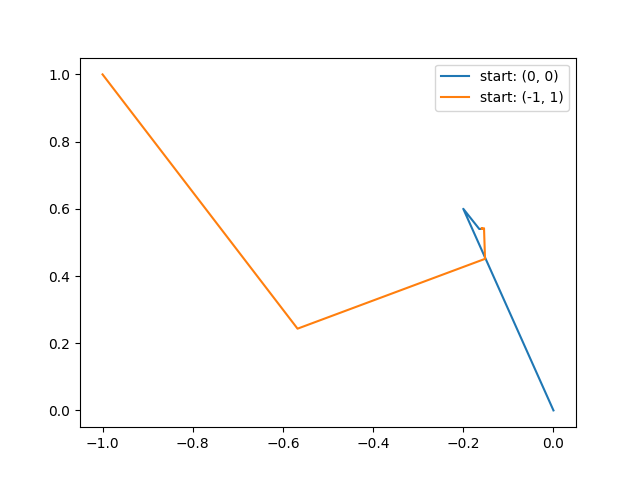
\includegraphics{iteration.png}
	\end{answer}
\end{document}